\section{Evaluations}
\label{evaluation}

In this section, we evaluate our proposed index structure for k-truss community queries on real-world networks.

%\subsection{Datasets}
\vskip 0.1in \noindent \textbf{Datasets} 

\begin{table}
		\caption{Datasets}
		\vspace{2 mm}
		\label{table:datasets}
		\begin{threeparttable}
			\centering
			\begin{tabular}{c|ccccc} \hline
				Dataset & Type & $|V_{wcc}|$ & $|E_{wcc}|$ & $|\triangle|$ & $k_{max}$ \\ \hline
				Wiki & Communication & 2.4M & 4.7M &  & \\ 
				Skitter & Internet & 1.7M & 11.1M & & \\ 
				Livejournal & Social & 4.8M & 43.4M & & \\ 
				Hollywood & Collaboration & 1.1M & 56.3M & & \\ 
				Orkut & Social & 3M & 117M & & \\ 
				Sinaweibo & Social & 58.7M & 261.3M & & \\ 
				Webuk & Web & 39.3M & 796.4M & & \\ 
				Friendster & Social & 65M & 1.8B & & \\ \hline
			\end{tabular}
			\begin{tablenotes}
				\item Datasets with the number of vertices and edges in the largest weakly connected components, the number of triangles and the maximum trussness of the graph.
			\end{tablenotes}
		\end{threeparttable}
\end{table}

We evaluate our algorithm on 8 graphs from different disciplines as shown in table~\ref{table:datasets}. To simplify our experiments, we treat them as undirected, un-weighted graphs and only use the largest weakly connected component of each graph. All datasets are collected from Stanford Network Analysis Project~\cite{snapnets} and Network Repository~\cite{nr-aaai15}.

%\subsection{Experiment settings}
\vskip 0.1in \noindent \textbf{Experiment settings} 

We evaluate our algorithms, we use a Cloudlab~\cite{RicciEide:login14} c8220 server with two 10-core 2.2GHz E5-2660 processors and 256GB memory. All algorithms are implemented in C++. 

\subsection{Query time}
\label{eval_query_time}

We evaluate the query time of various types of k-truss community queries on our index structure. We first evaluate the single vertex k-truss community search and compare the query time with the TCP index proposed in~\cite{huang2014querying}. Then we evaluate multi query vertices scenarios and show the results for k-truss query, max-k-truss query and any-k-truss query. Note that queries for exact truss communities can be executed by perform the centain truss community information query to get the id of the truss community first and then perform a BFS on \inducedgraph{}. The latter procedure is exactly same as the single vertex k-truss community search. Therefore we do not include it in our experiments.

\begin{figure}[ht]
    \centering
    %\includegraphics[width=\linewidth]{./figures/single_v_query_degree.pdf}
		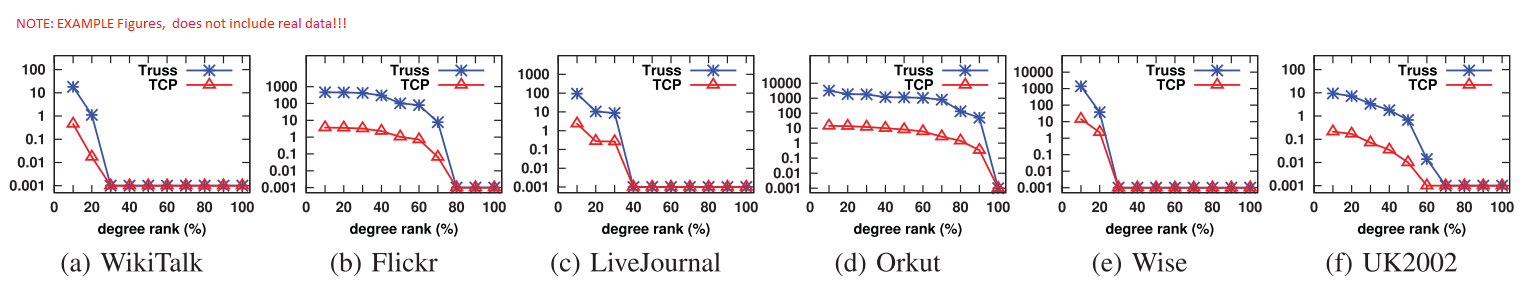
\includegraphics[width=\linewidth]{./figures/example.png}
    \caption{Single vertex query for exact truss community search.}
    \label{fig:single_v_query_degree}
\end{figure}

\begin{figure}[ht]
    \centering
			%\includegraphics[width=\linewidth]{./figures/single_v_query_k.pdf}
		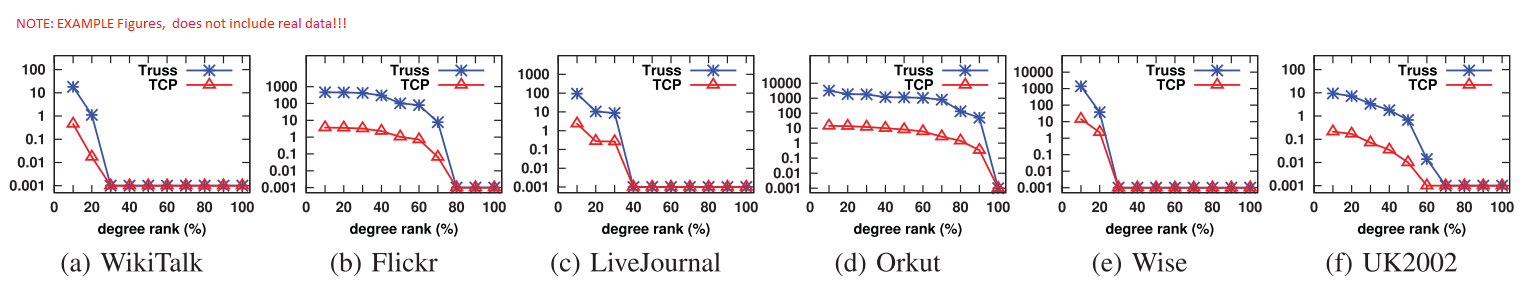
\includegraphics[width=\linewidth]{./figures/example.png}
    \caption{Single vertex query for exact truss community search.}
    \label{fig:single_v_query_k}
\end{figure}

For single vertex k-truss community search, in figure \ref{fig:single_v_query_k} and figure \ref{fig:single_v_query_degree}, we shows that our index outperforms the TCP index proposed in~\cite{huang2014querying}. We first fix k = 10 for all networks and show the k-truss community search time for vertices with various degrees on different graphs in figure \ref{fig:single_v_query_degree}. We can see that ... Then we use same set of vertices and show the results of various k on different graphs in figure \ref{fig:single_v_query_k}. We can see that ...
 
\subsection{Index construction time and size}
\label{eval_const}

\begin{table}
		\caption{Comparison of Index Construction}
		\vspace{2 mm}
		\label{table:index_construction}
		\centering
		\begin{tabular}{|c|c|cc|cc|} \hline 
			 & Graph & \multicolumn{2}{|c|}{Index Size} & \multicolumn{2}{|c}{Index Time} \\
			\cline{3-6}
			Dataset & Size & TCP  & Our & TCP & Our \\ \hline
			Wiki & 57 & 296 & 187 & 138 & 117\\ 
			Skitter & 149 & 485 & 430 & 873 & 682\\ 
			Livejournal & 635 & 3174 & 2699 & 1686 & 1557\\ 
			Hollywood & 791 & 4628 & 4012 & 4788 & 3966\\ 
			Orkut & 1769 & 8174 & 5742 & 3342 & 2884\\ 
			Sinaweibo & 4050 &  &  &  & \\ 
			Webuk & 13999 &   &  &  & \\ 
			Friendster & 32364 &   &  &  & \\ \hline
		\end{tabular}
\end{table}

We show in this section the index size and index construction time of our scheme compared to TCP-index in 
table \ref{table:index_construction}. Both indices are generated in memory and we show the size of the data structures that hold the index. We exclude the truss decomposition time for both scheme so that the index construction time only shows how long it takes to generate a certain index with edge trussness provided. 

We can see in table \ref{table:index_construction} that our scheme have smaller index size for most graphs and takes shorter time to generate the index compared to the TCP-index. The index size of our scheme is ... smaller than ...  The index construction time of our scheme is ... faster than ...

\subsection{Index update time}
\label{eval_update}

The index update time upon graph changes, i.e. edge deletion, is shown in ... 


